


\documentclass{article}
\usepackage{graphicx}
\begin{document}
\section*{Image processing with Python}

Working with images is an invaluable skill in scientific computing. There is so
much information hidden away in images that can be accessed with knowledge about
the right kind of tools and filters.
\newline \newline
Consider the image below:
\begin{figure}[h]
\begin{center}
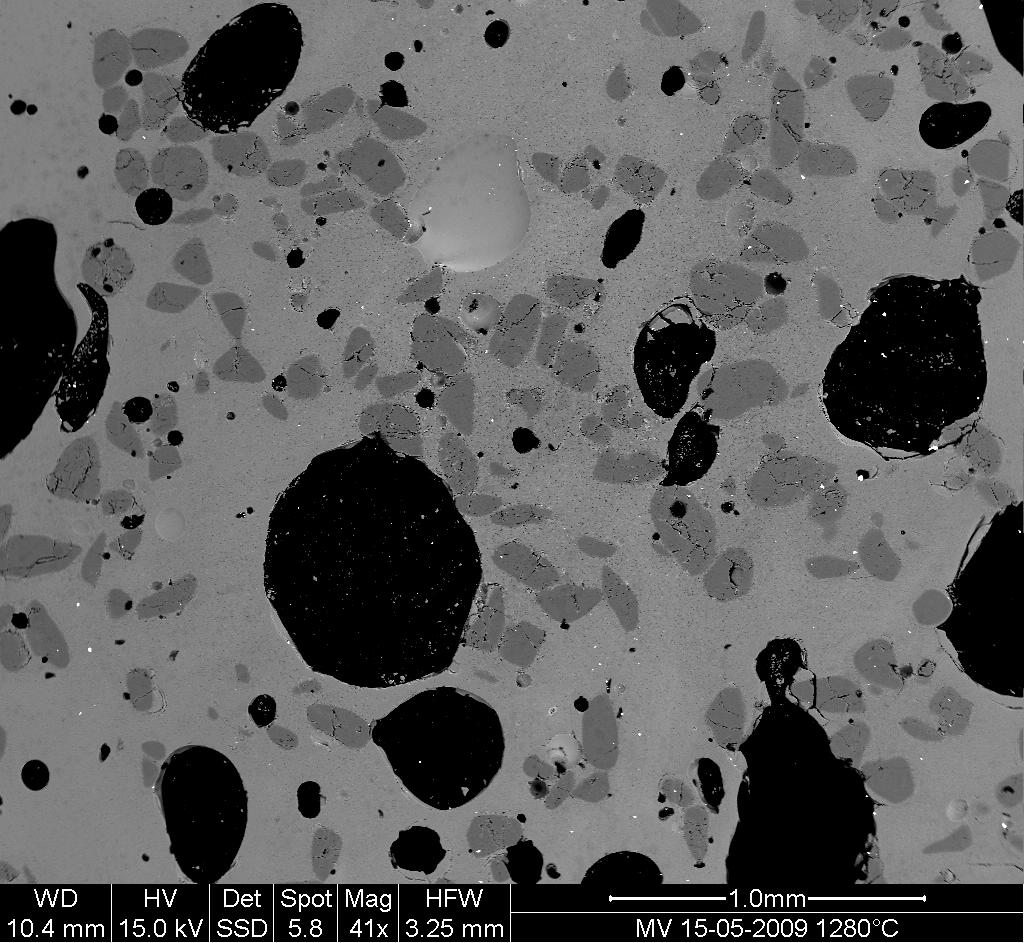
\includegraphics[width=150pt]{../pictures/MV_HFV_012.jpg}
\caption{SEM glass sample}
\end{center}
\end{figure}
\newline
This is an image of a sample of glass produced by a scanning electron microscope.
Visible in the image are three distinct ``phases'' : 
\begin{enumerate}
\item Glass matrix (light gray)
\item Unmolten sand particles (darker gray)
\item Voids/bubbles (black)
\newline
\end{enumerate} 
Your objectives are:
\begin{enumerate}
\item Determine the approximate fraction of each phase in the sample
\item Determine the average size of the voids
\end{enumerate} 
\end{document}
